\documentclass[a4paper, 12pt]{report}
\usepackage[T2A]{fontenc} 
\usepackage[utf8]{inputenc}
\usepackage[english,russian]{babel} 
\usepackage{amsmath,amsfonts,amssymb,amsthm,mathtools}
\usepackage[left=2cm,right=2cm,top=2cm,bottom=2cm,bindingoffset=0cm]{geometry}
\usepackage{graphicx}
\usepackage[linesnumbered,boxed]{algorithm2e}
\usepackage{verbatim}

\newenvironment{Proof} 
{\par\noindent{$\blacklozenge$}}
{\hfill$\scriptstyle\boxtimes$} 

\newenvironment{example} 
{\par\noindent{\textsc{\textbf{Пример}.}}} 
{\hfill$\scriptstyle\Box$} 

\newtheorem*{theorem}{Теорема} 
\newtheorem*{corollary}{Следствие}
\newtheorem*{lemma}{Лемма}

\newcommand{\RNumb}[1]{\uppercase\expandafter{\romannumeral #1\relax}}
\newcommand{\Rm}{\mathbb{R}}
\newcommand{\Cm}{\mathbb{C}}
\newcommand{\I}{\mathbb{I}}
\newcommand{\N}{\mathbb{N}}
\newcommand{\Z}{\mathbb{Z}}
\newcommand{\Q}{\mathbb{Q}}

\title{\textbf{\Huge{Методы вычислений}}\\Лабораторная работа 2\\«Решение СЛАУ с симметричными матрицами»\\Выполнила Николаева Ксения, 9 группа}
\date{} 

\begin{document}
    \maketitle

    \textbf{\Huge{Постановка задачи}}\\\\
        Разработать программу на C++, реализующую решение систем линейных алгебраических уравнений $( Ax = b )$ с симметричной матрицей на основе $LDL^T$-разложения. Использовать тип \textit{double}.\\
    Задача:\\
    Решить систему с симметричной матрицей $A$ порядка $n = 1000$, заполненной случайными числами от $-100$ до $100$ для $i < j$ и числами от $\sum_{j \neq i}|a_{ij}| + m$ до $\sum_{j \neq i}|a_{ij}| + 10m$.  Вектор точного решения $x$ задать как:
    \[
   x = \begin{pmatrix}
   m \\
   m + 1 \\
   \vdots \\
   m + n - 1
   \end{pmatrix}
   \]
   где $m = 8$ — номер студента. Правую часть $b$ вычислить как $b = Ax$.\\ 
   Вывести первые и последние 5 координат векторов $x$ и $ \tilde{x}$ (приближенное решение), а также относительную погрешность и время выполнения.\\
   

   \newpage
   \textbf{\Huge{Краткие теоретические сведения}}\\\\
   \textbf{Метод $LDL^T$-разложения} представляет матрицу $A$ в виде произведения трех матриц: $$A = L \dot D \dot L^T$$ где $L$ --нижняя треугольная матрица с единичными элементами на главной диагонали,  $D$ -- диагональная матрица\\\\
   \textbf{Формулы}
   $$A_{ii} = a_{ii} = \sum_{k = 1}^{i - 1}l_{ik}^2d_{kk}, i = 1, \dots n$$\\
   $$l_{ij} = \dfrac{1}{d_{jj}} \dot (a_{ij} - \sum_{k = 1}^{j - 1}l_{ik}  d_{kk}  l_{jk}), j = 1, \dots n - 1, i = j + 1, \dots n$$\\
   \textbf{Псевдокод}

   \begin{algorithm}
       
       \For{j = 1 ... n} {
       $d_{jj} = a_{jj} - sum_{k = 1}^{j - 1}l_{jk}^2d_{kk}$
       \For{i = j + 1 ... n} {
       $l_{ij} = \dfrac{1}{d_{jj}} \dot (a_{ij} - \sum_{k = 1}^{j - 1}l_{ik}  d_{kk}  l_{jk})$
       }
       }
       $Ly = b$\\
       $Dz = y$\\
       $L^Tx = z$\\\\
   \end{algorithm}
   \textbf{Погрешности в вычислениях}делятся на абсолютные и относительные\\
   $\bullet$ Абсолютная погрешность — это разность между истинным и вычисленным значениями\\
   $\bullet$ Относительная погрешность — отношение абсолютной погрешности к истинному значению:$$\delta =  \dfrac {||x - \tilde{x}||_{\infty}}{||x||_{\infty}}$$\\
   Метод Гаусса с выбором главного элемента помогает снизить ошибки округления, улучшая точность вычислений.\\

   \newpage
   \textbf{\Huge{Листинг программы с комментариями}}\\\\
   \begin{verbatim}
#include <bits/stdc++.h>
using namespace std;

const int N = 1e3 + 1;
const int M = 1e3 + 9;
const int MOD = 1e9 + 7;
const long long INF = 1e18 + 9;

vector<vector<long double>> A, A1;
vector<long double> b, b1;
vector<long double> x;
vector<long double> x1;

int n;
int m = 8;
bool can = 1;

///Создание матрицы A
void createMatrix(int n) {
    srand(time(0));
    for (int i = 0; i < n; ++i) {
        for (int j = i + 1; j < n; ++j) {
            A[i][j] = rand() % 201 - 100;
        }
    }
    for (int i = 0; i < n; ++i) {
        for (int j = 0; j < i; ++j) {
            A[i][j] = A[j][i];
        }
    }
    for (int i = 0; i < n; ++i) {
        int sum = 0;
        for (int j = 0; j < n; ++j) {
            if (i == j) continue;
            sum += abs(A[i][j]);
        }
        A[i][i] = rand() % (sum + 10 * m + 1) - (sum + m);
    }
}

///Вычисление значений вектора b
void createB(int n) {
    b.resize(n, 0);
    for (int i = 0; i < n; ++i) {
        for (int j = 0; j < n; ++j) {
            b[i] += A[i][j] * x[j];
        }
    }
}
///Метод Гаусса
void GaussianElimination(int n) {
    ///Прямой ход
    for (int i = 0; i < n - 1; ++i) {
        ///Столбец с максимальным элементом
        int maxRow = i;
        for (int k = i + 1; k < n; ++k) {
            if (fabs(A[k][i]) > fabs(A[maxRow][i])) {
                maxRow = k;
            }
        }

        if (fabs(A[maxRow][i]) < 1e-12) {
            cout << "It is impossible to solve the system:\nthe matrix is singular or close to singular in the row " << i + 1 << ".\n";
            can = 0;
            return;
        }
        swap(A[i], A[maxRow]);
        swap(b[i], b[maxRow]);
        for (int k = i + 1; k < n; ++k) {
            long double factor = A[k][i] / A[i][i];
            for (int j = i + 1; j < n; ++j) {
                A[k][j] -= factor * A[i][j];
            }
            b[k] -= factor * b[i];
        }
    }
    ///Обратный ход
    x1.resize(n);
    x1[n - 1] = b[n - 1] / A[n - 1][n - 1];
    for (int i = n - 2; i >= 0; --i) {
        x1[i] = b[i];
        for (int j = i + 1; j < n; ++j) {
            x1[i] -= A[i][j] * x1[j];
        }
        x1[i] /= A[i][i];
    }
}

///LDLt разложение
void LDLTDecomposition(int n) {
    vector<long double> D(n);
    vector<vector<long double>> L(n, vector<long double>(n, 0));

    for (int j = 0; j < n; ++j) {
        long double sum = 0;
        for (int k = 0; k < j; ++k) {
            sum += L[j][k] * L[j][k] * D[k];
        }
        D[j] = A[j][j] - sum;
        for (int i = j + 1; i < n; ++i) {
            sum = 0;
            for (int k = 0; k < j; ++k) {
                sum += L[i][k] * D[k] * L[j][k];
            }
            L[i][j] = (A[i][j] - sum) / D[j];
        }
    }
    /// Решение системы через разложение LDLT
    vector<long double> y(n), z(n);
    /// Решение L * y = b
    for (int i = 0; i < n; ++i) {
        long double sum = 0;
        for (int j = 0; j < i; ++j) {
            sum += L[i][j] * y[j];
        }
        y[i] = (b[i] - sum);
    }
    /// Решение D * z = y
    for (int i = 0; i < n; ++i) {
        z[i] = y[i] / D[i];
    }
    /// Решение L^T * x = z
    for (int i = n - 1; i >= 0; --i) {
        long double sum = 0;
        for (int j = i + 1; j < n; ++j) {
            sum += L[j][i] * x1[j];
        }
        x1[i] = z[i] - sum;
    }
}

///Вывод ответа для задачи
void printAnswer(int n) {
    cout << "Exact solution\n";
    for (int i = 0; i < 5; ++i) {
        cout << "x" << i + 1 << " = " << fixed << setprecision(15) << x[i] << '\n';
    }
    cout << "...\n";
    for (int i = n - 5; i < n; ++i) {
        cout << "x" << i + 1 << " = " << fixed << setprecision(15) << x[i] << '\n';
    }
    cout << "---------------------\n";
    cout << "Approximate solution\n";
    for (int i = 0; i < 5; ++i) {
        cout << "~x" << i + 1 << " = " << fixed << setprecision(15) << x1[i] << '\n';
    }
    cout << "...\n";
    for (int i = n - 5; i < n; ++i) {
        cout << "~x" << i + 1 << " = " << fixed << setprecision(15) << x1[i] << '\n';
    }
    ///Подсчет относительной погрешности
    cout << "---------------------\n";
    cout << "Relative error\n";
    long double max_diff = 0, max_exact = 0;
    for (int i = 0; i < n; ++i) {
        max_diff = max(max_diff, abs(x[i] - x1[i]));
        max_exact = max(max_exact, abs(x[i]));
    }
    long double relative_error = max_diff / max_exact;
    cout << scientific << setprecision(15) << relative_error << '\n';
}

int32_t main() {
    freopen("output.txt", "w", stdout);
    n = 1000;
    A.resize(n, vector<long double>(n));
    A1.resize(n, vector<long double>(n));
    b.resize(n);
    b1.resize(n);
    x.resize(n);
    x1.resize(n);
    createMatrix(n);
    A1 = A;
    for (int i = 0; i < n; ++i) {
        x[i] = m + i;
    }
    createB(n);
    b1 = b;
    ///Решение системы через разложение
    clock_t start = clock();
    LDLTDecomposition(n);
    clock_t end = clock();
    long double elapsed_time =  double(end - start) / CLOCKS_PER_SEC; ///подсчет затраченного времени
    printAnswer(n);
    cout << "Time LDLT Decomposition: " << elapsed_time << " seconds\n";
    ///Вычисление времени для решения аналогичной задачи Методом Гаусса
    A = A1;
    b = b1;
    start = clock();
    GaussianElimination(n);
    end = clock();
    elapsed_time =  double(end - start) / CLOCKS_PER_SEC; ///подсчет затраченного времени
    cout << "Time Gaussian Elimination: " << elapsed_time << " seconds\n";
    return 0;
}
   \end{verbatim}
   \newpage
   \textbf{\Huge{Результаты}}\\\\
   $\bullet$ Результат вычислительного экперимента для задачи с матрицей $A$ порядка $n = 1000$\\
   \begin{center}
        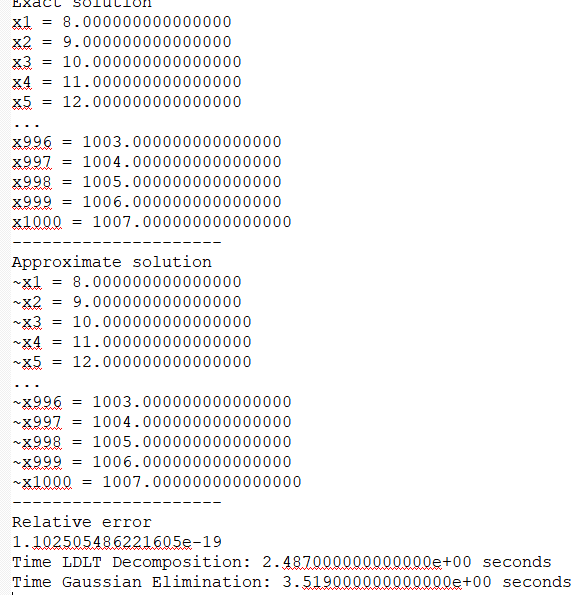
\includegraphics[scale = 0.7]{pic4.png}
   \end{center}
   

    \newpage
   \textbf{\Huge{Выводы}}\\\\
      $\bullet$ Использование $LDL^T$-разложения для решения систем линейных уравнений с симметричной матрицей показало свою эффективность. Этот метод особенно хорошо подходит для таких задач, поскольку он учитывает структуру симметричной матрицы, что позволяет снизить количество вычислений по сравнению с более универсальными методами, такими как метод Гаусса.\\
   $\bullet$ Время выполнения программы с использованием $LDL^T$-разложения было сравнено с временем, затраченным на решение аналогичной задачи с использованием метода Гаусса (лабораторная работа №1).$LDL^T$-разложение показало лучшую производительность на симметричных матрицах, что подтверждает его эффективность для такого типа систем.\\
   $\bullet$ Относительная погрешность между точным и приближённым решениями оказалась низкой, что свидетельствует о высокой точности метода $LDL^T$-разложения при решении крупных систем линейных уравнений с симметричной матрицей.\\
   
\end{document}


